\section{Modeling of Ablating Thermal Protection Systems}

This section presents the ablation problem for a non-decomposing TPS as a parametrized system of non-linear PDEs. These non-linear PDEs govern the energy of heat conduction and the pseudo-elastic material deformation of the mesh motion. Two different but mathematically-connected numerical solution strategies are provided: (1) a high-fidelity full-order model (FOM) based on a discontinuous Galerkin FEM, and (2) a thermo-elastic RPM based on a one-dimensional approximation to the energy and pseudo-elasticity equations.

\subsection{Governing Equations}\label{sec_governing_equations}

Consider a generic domain $\Omega\subset$, $d=2$ or $3$, illustrated in Fig.~\ref{fig_general_domain}. A heat flux $q_b(x,t)$ is prescribed on the boundary $\Gamma_q$ (i.e., Neumann boundary condition), and the temperature $T_b(x,t)$ is prescribed on boundary $\Gamma_T$ (i.e., Dirichlet boundary condition), where $\Gamma_q\cup\Gamma_T = \partial\Omega$ and $\Gamma_q\cap\Gamma_T = \emptyset$. The ablation occurs only on the heated boundary $\Gamma_q$, and its effects are included into the energy equation using an Arbitrary Lagrangian-Eulerian (ALE) description. The ALE assumes that the displacement $\vw(x,t)\in\mathbb{R}^d$ of the computational mesh moves with velocity $\vv(x,t)$ that is different to the material velocity, which is fixed to zero in this work.

\begin{figure}
    \centering
    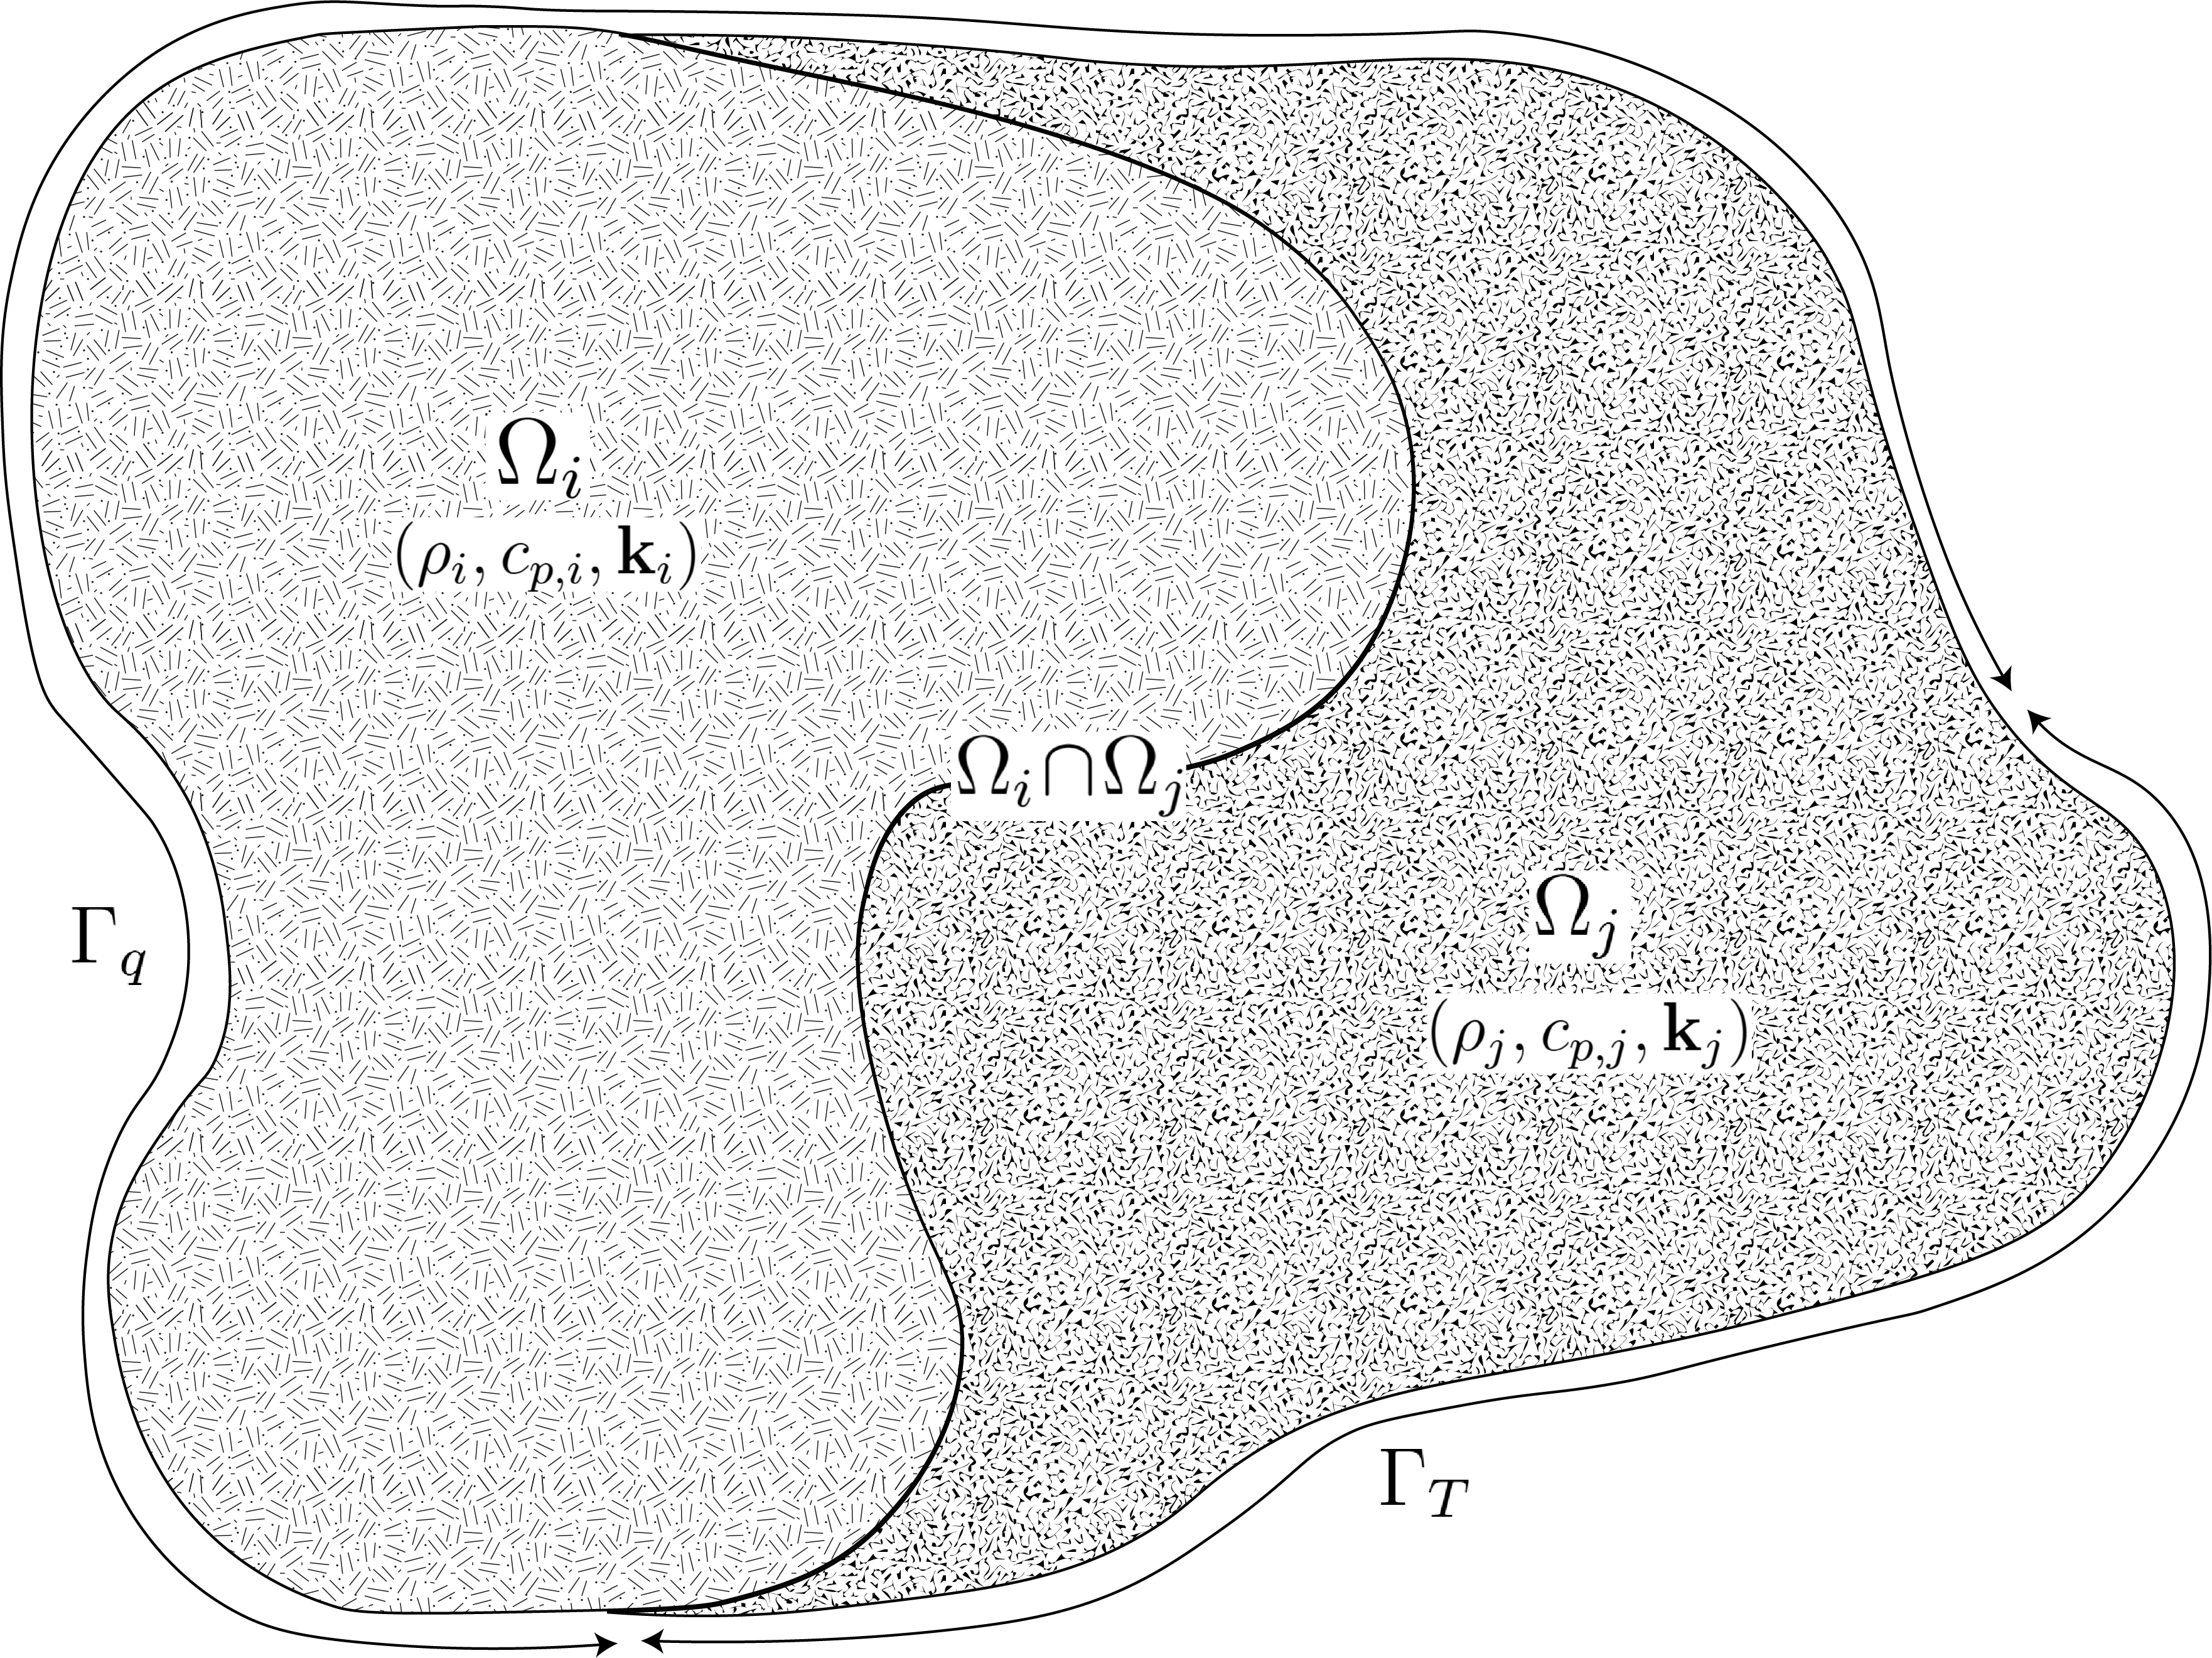
\includegraphics[width=0.6\textwidth]{./figs/general_domain.png}
    \caption{General domain $\Omega$ with prescribed heat flux $q_b(x,t)$ and temperature $T_b(x,t)$ on the boundaries $\Gamma_q$ and $\Gamma_T$, respectively. The mesh moves with a velocity $\mathbf{v}(x,t)$, while the material velocity is $\mathbf{w}(x,t)$.\hl{draw mesh next to arbitrary domain with moving boundaries.}}
    \label{fig_general_domain}
\end{figure}

The transient heat conduction over the moving mesh is described by the following equations,
\begin{subequations}
    \begin{align}
        \rho c_p\left(\ppt{T} - \mathbf{v}(x,t)\cdot\nabla T\right) - \nabla\cdot (\mathbf{k}\nabla T) &= \cQ(x,t),\ x\in\Omega \label{eqn_thermal_pde}\\
        \nabla\cdot\boldsymbol{\sigma}(\mathbf{w}) &= 0\label{eqn_elasticity_pde}\\
        -\mathbf{k}\nabla T\cdot \vn &= q_b(x,t),\ x\in\Gamma_q\label{eqn_thermal_bc_neumann}\\
        T(x,t) &= T_b(x,t),\ x\in\Gamma_T\label{eqn_thermal_bc_dirichlet}\\
        T(x,0) &= T_0(x),\ x\in\Omega\label{eqn_thermal_ic}\\
        \vw(x,t) &= \vw_q(x,t),\quad x\in\Gamma_q\label{eqn_displacement_heated_bc}\\
        \vw(x,t) &= 0,\quad x\notin \Gamma_q\label{eqn_displacement_unheated_bc}\\
        \vw(x,t) &= \boldsymbol{0}\label{eqn_displacement_initial_condition}
    \end{align}\label{eqn_governing_equations}
\end{subequations}
The density $\rho$, heat capacity $c_p$, and thermal conductivity $\mathbf{k}\in\mathbb{R}^{n_d\times n_d}$ are assumed to be constant with respect to temperature in this work. The terms in \cref{eqn_thermal_pde}, in the order they appear, correspond to the unsteady energy storage, heat conduction, temperature advection due to mesh motion, and the heat source terms. 

The elasticity equation \cref{eqn_elasticity_pde} states that the divergence of the stress tensor $\boldsymbol{\sigma}(\mathbf{w})$ is zero. The stress tensor is related to the strain tensor $\bepsilon(\bw)$ through Hooke's law,
\[
    \boldsymbol{\sigma}(\bw) = \mathbb{D}:\boldsymbol{\epsilon}(\bw)
\]
where $\mathbb{D}$ is the constitutive operator, ``:'' is the double contraction of tensors, and $\bepsilon$ is the symmetric strain tensor given by,
\[
    \bepsilon(\bw) = \frac{1}{2}\left(\nabla\bw + \nabla\bw^T\right)
\]
For instance, an isotropic material assumption results in,
\[
    \bsigma = \lambda\left(\nabla\cdot\bw\right) \mathbf{I} + 2\mu\bepsilon(\bw)
\]
where $\lambda$ and $\mu$ are Lame constants that are arbitrarily selected to model the mesh motion. The ``material'' properties $\lambda$ and $\mu$ can be chosen to tailor the mesh deformation and need not represent the actual material being modeled~\hl{Amar2016}. 

The boundary conditions for the energy equation includes a heated surface (\cref{eqn_thermal_bc_neumann}) and a constant-temperature surface (\cref{eqn_thermal_bc_dirichlet}). The boundary conditions for the pseudo-elasticity equation are a function of the surface temperature $T_q(x,t)$ for $x\in\Gamma_q$ using a B' table. The B' table....
\begin{equation}
    \bw_q(x,t) = \int_{0}^{t} \mathbf{v}(x,\tau)d\tau = \int_{0}^{t}\mathbf{f}\left(T_q(x,\tau)\right)d\tau\label{eqn_boundary_displacement}
\end{equation}


\subsection{Full-Order Model: Discontinuous Galerkin Finite Element Method}\label{sec_fom}

To obtain the full-order numerical solution, the governing equation is spatially discretized using variational principle of Discontinuous Galerkin (DG) to result in a high-dimensional system of ODEs for the time-varying nodal data. The full-order TPS ablation simulations are computed using standard FEM instead, and the equivalence between DG and standard FEM is noted upon their convergence.

Consider a conforming mesh partition domain, where each element belongs to one and only one component. Denote the collection of all $M$ elements as $\left\{E_i\right\}_{i=1}^{M}$. In an element $E_i$, its shared boundaries with another element $E_j$, Neumann BC, and Dirichlet BC are denoted as $e_{ij}$, $e_{iq}$, and $e_{iT}$, respectively. Lastly, $\left|e\right|$ denotes the length $(n_d=2)$ or area $(n_d=3)$ of a component boundary $e$.

For the $e$-th element, use a set of $n^{(e)}$ trial functions, such as polynomials, to represent the temperature distribution,
\begin{equation}
    T^{(e)}(x,t) = \sum_{i=1}^{n^{(e)}} \phi_i^{(e)}(x)u_i^{(e)} \equiv \boldsymbol{\phi}^{(e)}(x)^T\vu^{(e)}(t)
\end{equation}

\subsubsection{Numerical Solution}

\subsubsection{Usage Within an Ablation Simulation}


\subsection{Reduced-Physics Model: One-Dimensional Thermo-Elastic Solver}

In this section, the main results regarding the derivation of the thermo-elastic RPM are presented, with the details provided in Appendix~\hl{x}. The thermo-elastic RPM is derived to model the one-dimensional temperature distribution and surface recession for an ablating TPS. The temperature is modeled using a coarse-grained DG-FEM approach, while the moving mesh is modeled using an analytical solution to the elasticity equations.

Consider the partitioning of the general domain depicted in Fig.~\ref{fig_general_domain} into $N=3$ non-overlapping inter-connected components $\left\{\Omega_i\right\}_{i=1}^{3}$, as illustrated in Fig.~\ref{fig_domain_partition}. The coupling between the components is due to the volumetric energy source terms,
\[
    \cQnet^{(1)}(x,t),\quad\cQnet^{(2)}(x,t),\quad \cQnet^{(3)}(x,t)
\]
which are space-time varying, and are unknown quantities due to the moving interfaces between the interconnected components.


where the thermodynamic coupling occurs due to $\cQ^{(1,2)}(x,t)$ and $\cQ^{(2,3)}(x,t)$, which are space-time varying. The $i$-th component $\Omega_i$ is associated with material properties $\left\{\rho^{(i)}, c^{(i)}_{p}, k^{(i)}\right\}$, which are continuous within each component, and may be discontinuous across two neighboring components.

\begin{figure}
    \centering
    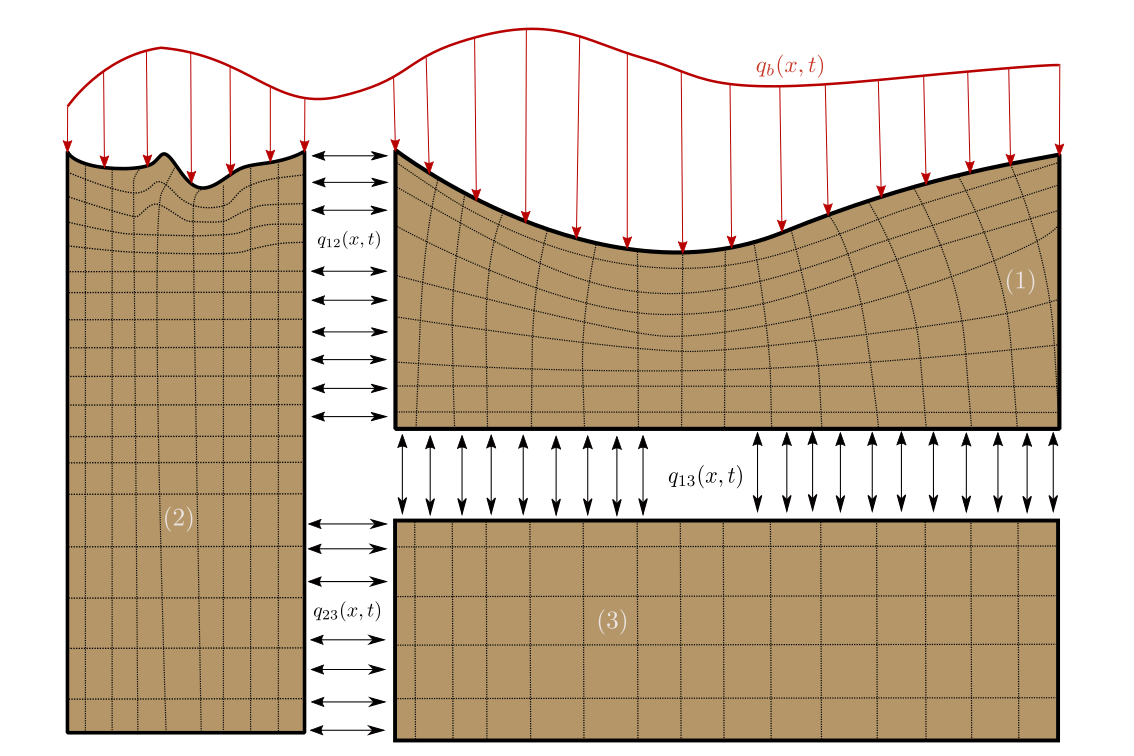
\includegraphics[width=0.8\textwidth]{./figs/three_components.png}
    \caption{Partition of the TPS into three one-dimensional components.}
    \label{fig_domain_partition}
\end{figure}

A first-order DG-FEM scheme is adopted for each component, with the coupling between the components enforced via interior point penalty methods~\hl{x} as discussed in Sec.~\ref{sec_fom}. The RPM results in a block-diagonal system of ODEs for the nodal temperature values on the three components, and is given as,
\begin{equation}
    \vA\left(\vu\right)\dot{\vu} + \left(\vB - \vC(t)\right)\vu = \mathbf{f}(t)\label{eqn_rpm}
\end{equation}
where the block matrices are defined as,
\begin{equation}
    \vA_{ij} = \left\{\begin{matrix}
        \vA^{i}(\vu^{(i)}),\quad i=j\\
        0,\quad i\neq j
    \end{matrix}\right.,\quad \vB_{ij} = \left\{\begin{matrix}
        \vB^{(i)}(\vu^{(i)}),\quad i=j\\
        0,\quad i\neq j
    \end{matrix}\right.
\end{equation}
The details involving the RPM derivation are provided in Appendix.

The ablation on the $i$-th component is modeled using a one-dimensional approximation to the temperature and mesh-motion equations in \cref{eqn_governing_equations}, and are given by,
\begin{subequations}
    \begin{align}
        \rho c_p\left(\frac{\partial T^{(i)}}{\partial t} - v^{(i)}(x,t)\frac{\partial T^{(i)}}{\partial x}\right) - \frac{\partial}{\partial x}\left(k\frac{\partial T^{(i)}}{\partial x}\right) - \cQ^{(i)}_{\text{net}}(x,t) &= 0\label{eqn_thermal_1d}\\
        \frac{\partial}{\partial x}\left(\frac{\partial u^{(i)}}{\partial x}\right) &= 0\label{eqn_elasticity_1d}
    \end{align}\label{eqn_rpm}
\end{subequations}
with boundary conditions for the energy equation,
\begin{subequations}
    \begin{align}
        -k\frac{\partial T^{(i)}}{\partial x}\Bigg|_{x=0} &= q^{(i)}_b(t)\\
        -k\frac{\partial T^{(i)}}{\partial x}\Bigg|_{x=\ell} &= 0
    \end{align}
\end{subequations}
and for the elasticity equation,
\begin{subequations}
    \begin{align}
        u^{(i)}(0,t) &= \int_{t_0}^{t}v^{(i)}(\tau)d\tau = \int_{0}^{t} f(T^{(i)}_w(\tau))d\tau\\
        u^{(i)}(\ell,t) &= 0
    \end{align}
\end{subequations}
where $v^{(i)}(t)$ is the surface receding velocity due to ablation, which is a function of the surface temperature as in \cref{eqn_boundary_displacement}. The surface velocity is computed from a cubic spline interpolate to a B' look-up table...

The coupling between the one-dimensional strands is enforced through the net volumetric energy source term $\cQ^{(i)}_{\text{net}}$, which is computed as,
\begin{equation}
    \cQ^{(i)}_{\text{net}}(x,t) = \sum_j\cQ^{(i)}_{\text{in},j}(x,t) - \sum_j\cQ^{(i)}_{\text{out},j}(x,t)\label{eqn_net_volumetric_energy}
\end{equation}
For example, in the $i=2$ component of Fig.~\hl{x}, the net volumetric energy source term is,
\begin{subequations}
    \begin{align}
        \cQ^{(2)}_{\text{net}}(x,t) &= \sum_j\cQ^{(2)}_{\text{in},j}(x,t) - \sum_j\cQ^{(2)}_{\text{out},j}(x,t)\notag\\
        &= \cQ^{(1,2)}(x,t) - \cQ^{(2,3)}(x,t)
    \end{align}
\end{subequations}
In this work, the volumetric energy source term between the $i$-th and $j$-th components is approximated as,
\begin{equation}
    \cQ^{(i,j)}(x,t) = \frac{T^{(j)}(x,t) - T^{(i)}(x,t)}{R_{ij}}\label{eqn_volumetric_energy_approximation}
\end{equation}
where $R_{ij}$ is the so-called thermal resistance. Empirically, for a component of isotropic heat conductivity $k$, length $L$ and cross-section $A$, the thermal resistance is $R=L/kA$ . Between components $i$ and $j$, define $R_{ij} = R_i + R_j$.

Along the one-dimensional domain, a numerical solution based on FEM is adopted for the energy equation, while an analytical solution is adopted for the pseudo-elastic mesh motion. The quasi-steady boundary conditions for the mesh motion are employed via a spline fit to the B' and enthalpy tabulated data as a function of surface temperature. The main results of the numerical approach are presented here and the reader is directed to Sec.~\ref{app_implementation} for details.

\subsubsection{Thermal Solver}

The FEM implementation details are supplied in Appendix~\hl{x}. For the $n$-th component, the result of the FEM discretization is a system of ODEs for the nodal temperatures, coupled to the neighboring component $n+1$ through the energy volumetric source term,
\begin{equation}
    \mathbf{A}^{(i)}\frac{d\mathbf{T}^{(i)}}{dt} + \left(\mathbf{B}^{(i)} - \mathbf{C}^{(i)}(t)\right)\mathbf{T}^{(i)} = \mathbf{f}^{(i)}(t)
\end{equation}
where,
\begin{itemize}
    \item $\mathbf{A}^{(i)}\in\mathbb{R}^{M\times M}$ is the mass matrix,
    \item $\mathbf{B}^{(i)}\in\mathbb{R}^{M\times M}$ is the stiffness matrix,
    \item $\mathbf{C}^{(i)}(t)\in\mathbb{R}^{M\times M}$ is the advection matrix,,
    \item $\mathbf{T}^{(i)}\in\mathbb{R}^{M}$ is the vector of nodal temperatures, and
    \item $\mathbf{f}^{(i)}(t)\in\mathbb{R}^{M}$ is the input vector, which includes the Neumann boundary conditions and the net volumetric energy source term $\cQ^{(i)}_{\text{net}}$.
\end{itemize}
where $M$ is the number of nodes in the one-dimensional mesh for the $i$-th component.

\subsubsection{Pseudo-Elastic Solver}

Note that \cref{eqn_elasticity_1d} is steady. Under the assumption that the mesh deformation is quasi-steady, it can be applied at each time step within an ablation simulation. For instance, a known value of the wall temperature $T_w(t)$ specifies a Dirichlet boundary condition for the displacement, and the resulting nodal displacements within the ablator are determined from \cref{eqn_elasticity_pde}.

Along the one-dimensional domain, the PDE in \cref{eqn_elasticity_pde} simplifies to,
\begin{equation}
    \frac{\partial^2 u^{(e)}}{\partial x^2} = 0
\end{equation}
which has the analytical solution,
\begin{equation}
    u^{(e)}(x,t) = a(t)x + b(t)
\end{equation}
Imposing the boundary conditions leads to,
\begin{equation}
    u^{(e)}(x,t) = u^{(e)}(0,t)\left(\frac{x_1^{(e)} - x}{h^{(e)}}\right)
\end{equation}
The mesh velocity is the time derivative of the displacement,
\begin{equation}
    v^{(e)}(x,t) = \frac{\partial u^{(e)}(x,t)}{\partial t} = v^{(e)}(t)\left(\frac{x_1^{(e)} - x}{h^{(e)}}\right)
\end{equation}

\subsubsection{Coupling Scheme}

\subsubsection{Reduced-Physics Ablation Simulation}







